\section{VoLTE抓包结果分析}
\label{chap:analyze:results}

%通过抓包测试,得到了一些VoLTE视频流结果
在进行检测之前,首先要构造参照标准数据集。为得到有效数据,以三星A5108手机为平台,在多种网络场景下,进行了一些列视频通话测试。并通过tcpdump抓包软件\nupcite{10.5555/1047846.1047873},捕获了所有的视频数据包,用于后续的分析。

%分析抓包结果,对特征进行分析
\insertTable{
	\begin{table}[]
        \centering
        \caption{VoLTE视频通话抓包结果}
        \label{tab:3:capture-results}
        \begin{threeparttable}
            \begin{tabular*}{0.8\textwidth}{@{\extracolsep{\fill}}ccccc}
            \toprule
            场景 & 通话次数 & 数据包总数 & 抓包总数 & 平均丢包率 \\ 
            \midrule
            Excellent & 13 & 323297 & 320990 & 0.71\% \\ 
            Good & 17 & 288592 & 261470 & 9.4\% \\
            \bottomrule
            \end{tabular*}
            \begin{tablenotes}
                \footnotesize
                \item[] 视频数据包发送速率,约为100 pkts/s
            \end{tablenotes}
        \end{threeparttable}
    \end{table}
}
如表\nref{tab:3:capture-results},抓包场景分为两种。Excellent场景对应的是同基站内通话,及稳定网络下的通话;Good场景对应的是移动状态下的通话,以及跨基站通话。Excellent场景中,通话质量及流畅度均具有极佳表现;Good场景中,偶尔存在卡顿或图像模糊。这两种测试场景,对时间隐通道有不同的要求,后续将进行详细分析。

\subsection{丢包率}
\label{chap:analyze:results:plr}

%本节主要从丢包率进行分析,包括两个方面
丢包率是网络质量分析中,常用的评估指标,平均丢包率反映了网络信道的可靠性及稳定性。
%什么是全局丢包率
如表\nref{tab:3:capture-results},网络噪声导致的丢包,在不同场景下差异很大,无法支撑时间隐通道的检测需求。
%什么是区间丢包率
本文中结合区间丢包率进行分析,也就是将传输过程划分为定长的传输阶段,统计个区间丢包数量的分布。

\subsubsection{全局丢包率}
\label{chap:analyze:results:plr:global}

%统计的各个通话的全局丢包率,分布情况
\insertFigure{
	\begin{figure}
		\centering
        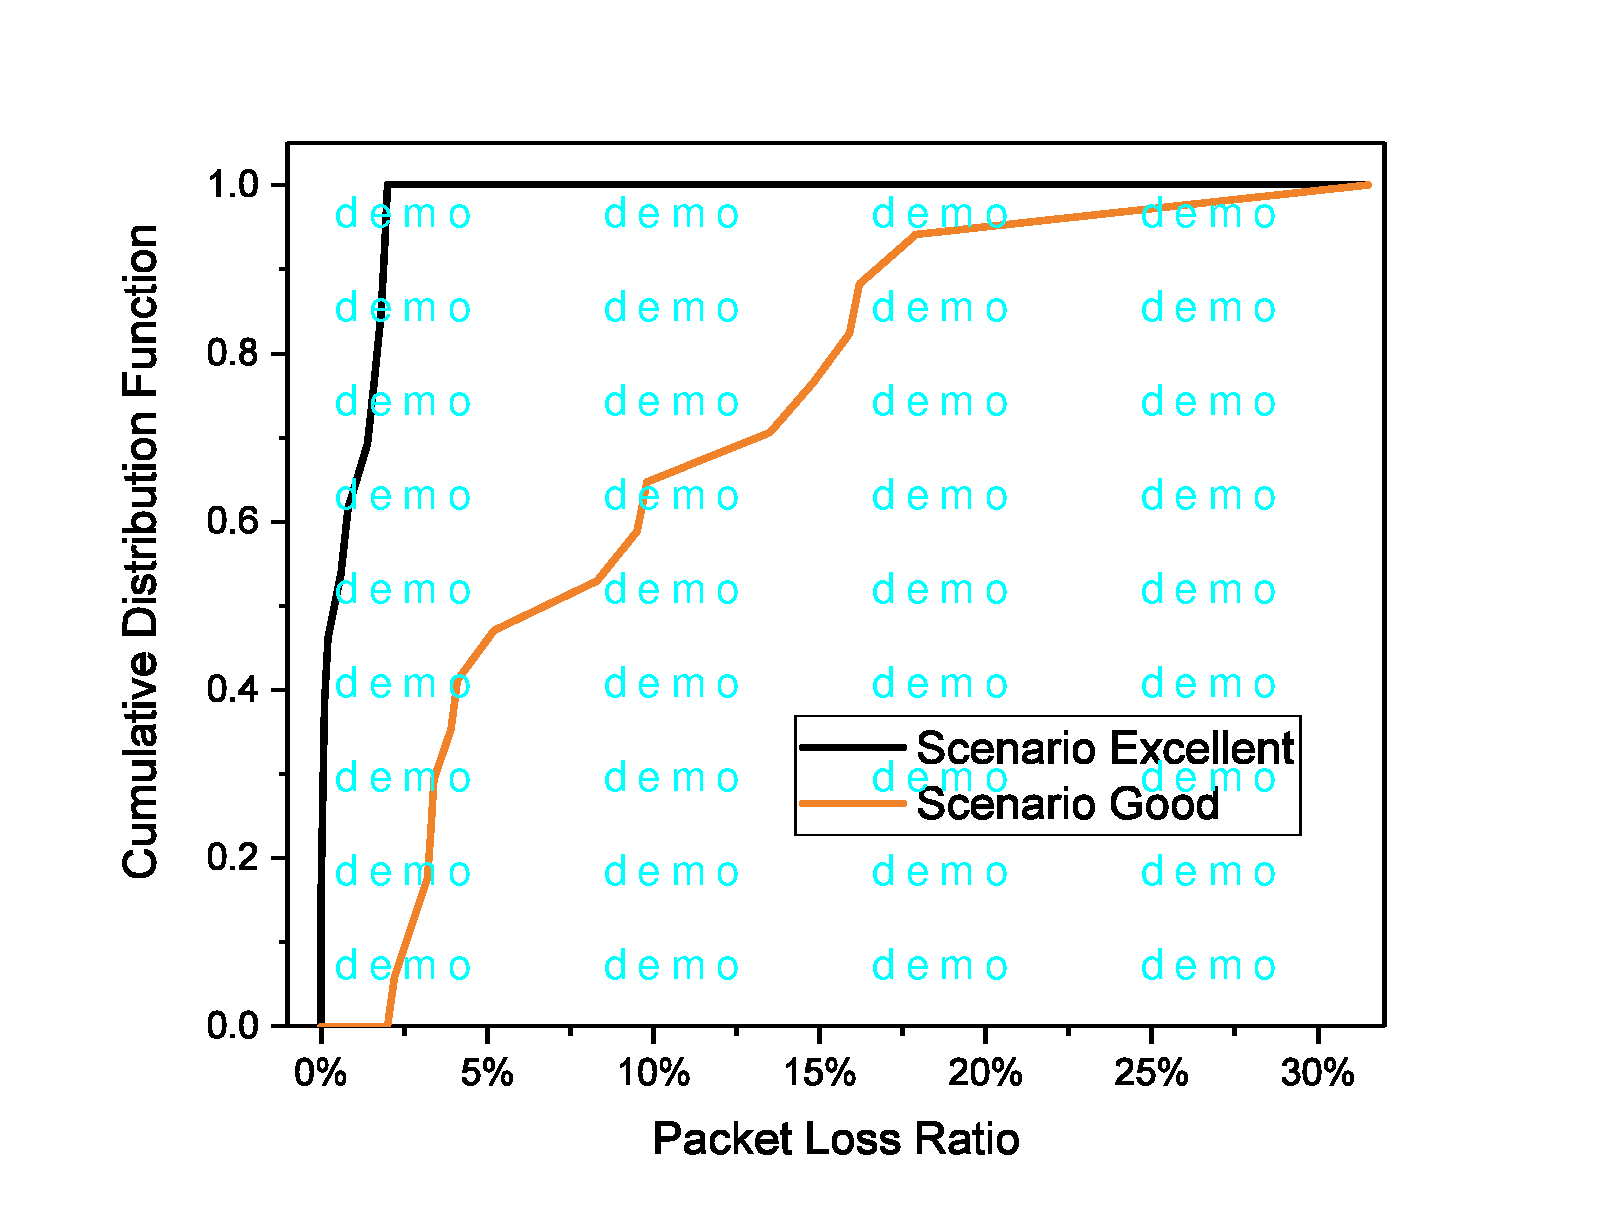
\includegraphics[width=0.8\textwidth]{chapters/chapter3/figures/capture-cdf-plr.pdf}
        \caption{两种场景中平均丢包率的累积分布图}\label{fig:3:cdf-plr}
	\end{figure}
}

如图\nref{fig:3:cdf-plr},两种场景平均丢包率的累积分布,出现明显的分离。Excellent场景下丢包率普遍较低,对时间隐通道的存在更敏感;Good场景中噪声干扰严重,丢包率显著上升,时间隐通道的检测难度增大。

\subsubsection{区间丢包数量}
\label{chap:analyze:results:plr:window}

%测试区间设定,以及不同场景下,各个区间的分布函数
区间丢包数量的测试方法,将数据包流按照设定的窗口大小划为区间,每个区间单独统计丢包数量。最终对各区间的丢包数量进行汇总,计算统计结果的累积分布。如图\nref{fig:3:win-size-count},在相同丢包状态下,通过控制窗口的大小,每个分片内的丢包数量,随着窗口增大而增加。

\insertFigure{
	\begin{figure}
		\centering
        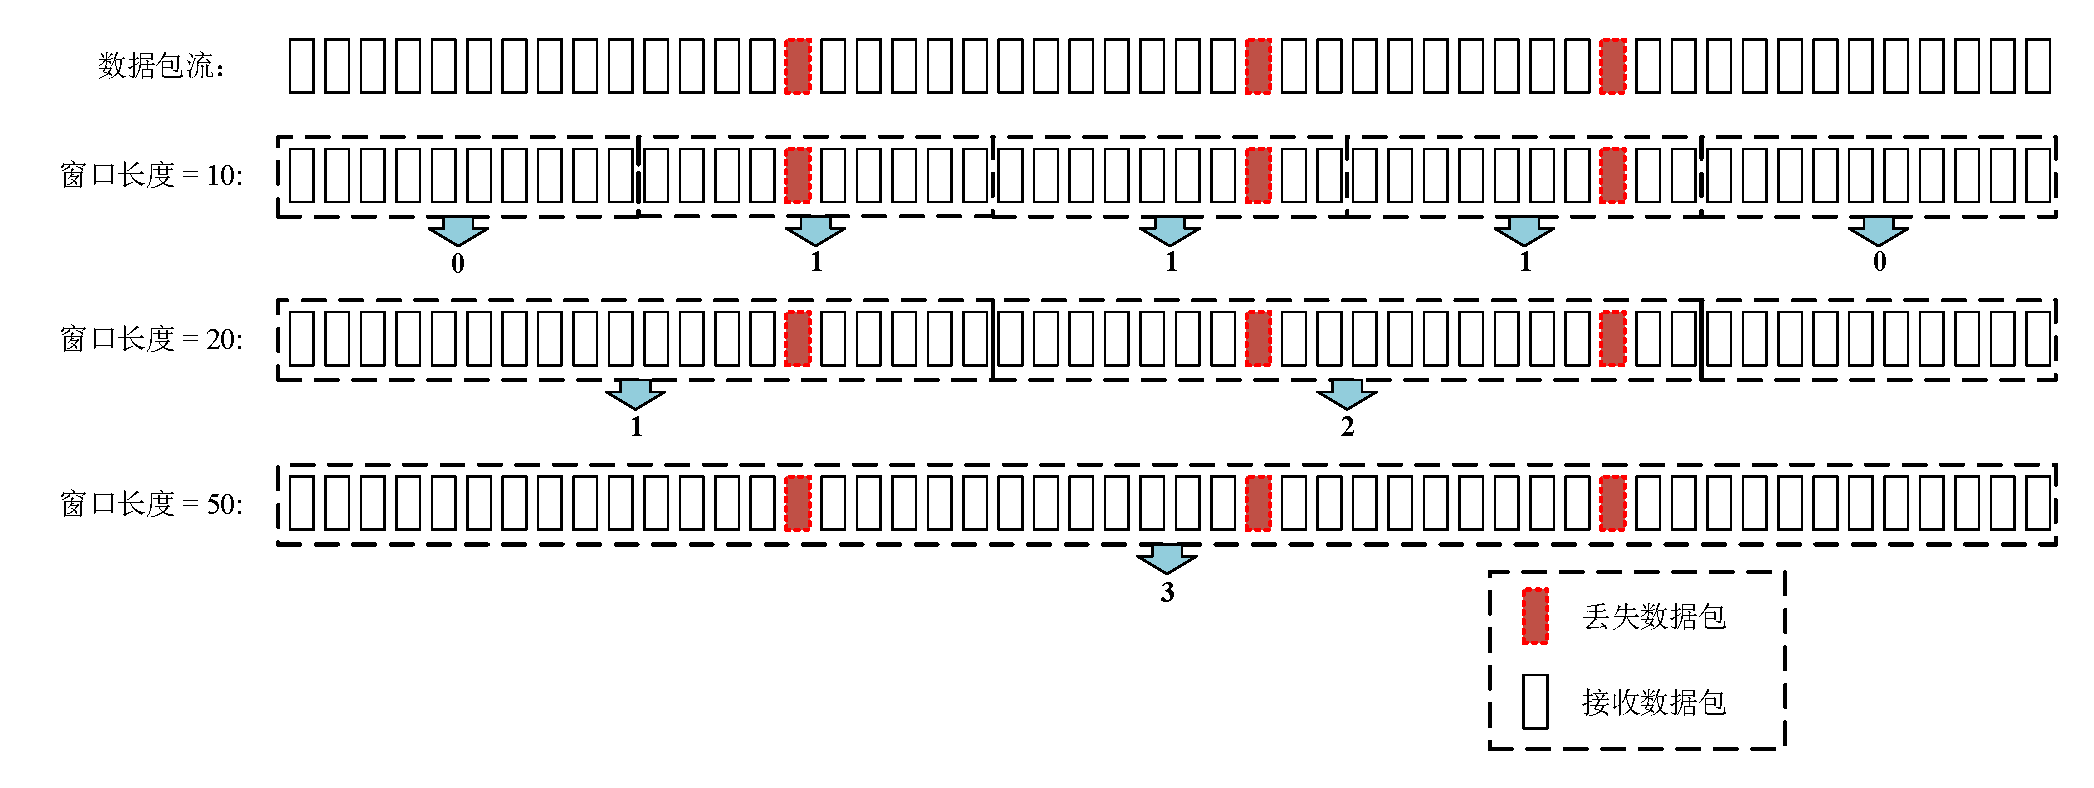
\includegraphics[width=0.99\textwidth]{chapters/chapter3/figures/win-size-count.pdf}
        \caption{窗口大小与丢包个数统计的示意图}\label{fig:3:win-size-count}
	\end{figure}
}

\insertFigure{
    \begin{figure}
    \centering
        \subfigure[Excellent场景下CDF结果]{
            \label{fig:3:capture:win-cdf:excellent}
            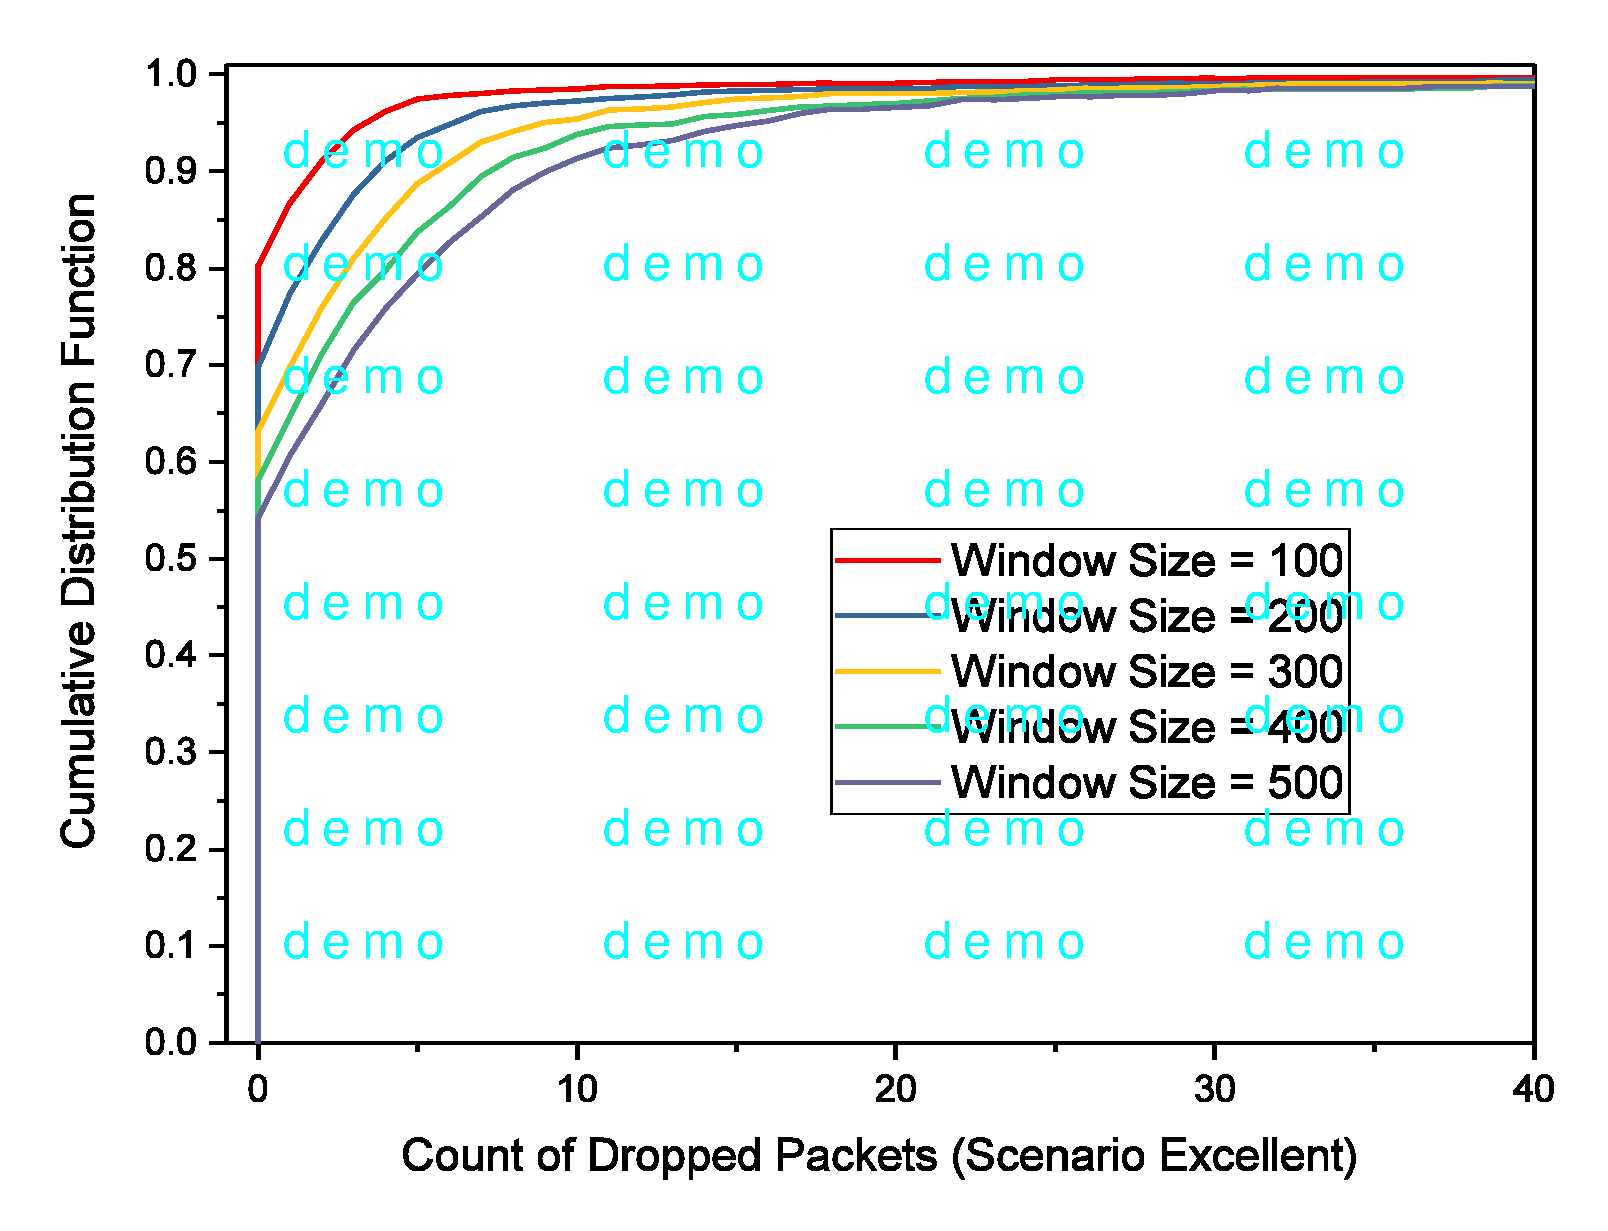
\includegraphics[width=0.48\textwidth]{chapters/chapter3/figures/capture-cdf-win-excellen.pdf}
        }
        \subfigure[Good场景下CDF结果]{
            \label{fig:3:capture:win-cdf:good}
            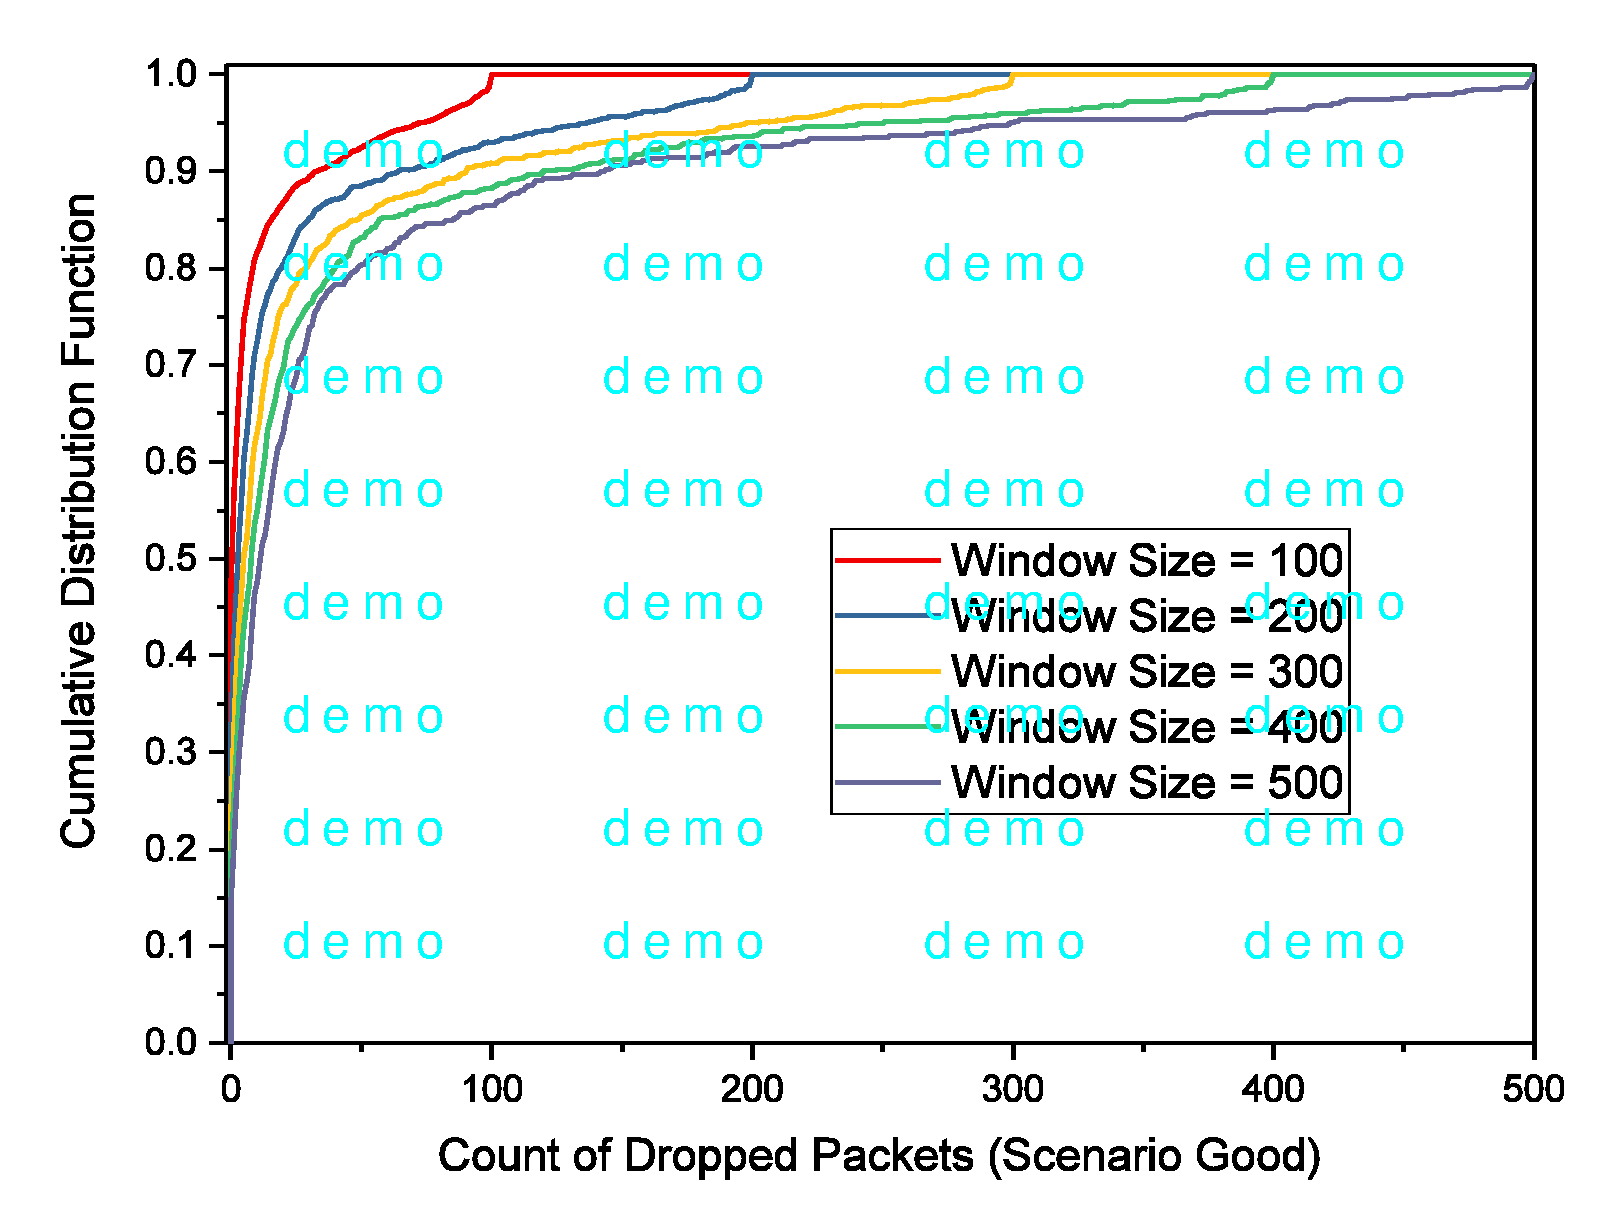
\includegraphics[width=0.48\textwidth]{chapters/chapter3/figures/capture-cdf-win-good.pdf}
        }
    \caption{两种场景中区间丢包数的累积分布函数}
    \label{fig:3:capture:win-cdf}
    \end{figure}
}

如图\nref{fig:3:capture:win-cdf},两种场景下的分布既存在总体相似性,局部特征中存在差异。图\nref{fig:3:capture:win-cdf:excellent}中,对于所有的窗口大小来说,丢包数量为0的区间均占据一半以上,并且CDF收敛到$1.0$的速度快,上升趋势明显且平滑,侧面反应网络质量极佳。图\nref{fig:3:capture:win-cdf:good}中,曲线上升趋势与图\nref{fig:3:capture:win-cdf:excellent}类似,但在丢包位置为0的部分比例较小,且在CDF曲线末尾仍有分布,证明存在数据包全丢的区间。

\subsection{数据包传输间隔}
\label{chap:analyze:results:ipd}

%IPD代表了什么
IPD分布是时间隐通道中的经典测试对象,如图\nref{fig:2:cdf-ipd},发送阶段的IPD分布与接收阶段的IPD分布,存在着明显的差异。发送阶段有两个集中分布的位置,而接收阶段曲线变为平滑,证明网络的缓冲及中转削弱了原始IPD的特征,接收方观测到的IPD接近正偏态分布。

%两种场景下抓包得到的IPD分布
\insertFigure{
    \begin{figure}
    \centering
        \subfigure[IPD分布的累积分布函数图]{
            \label{fig:3:capture:ipd:cdf}
            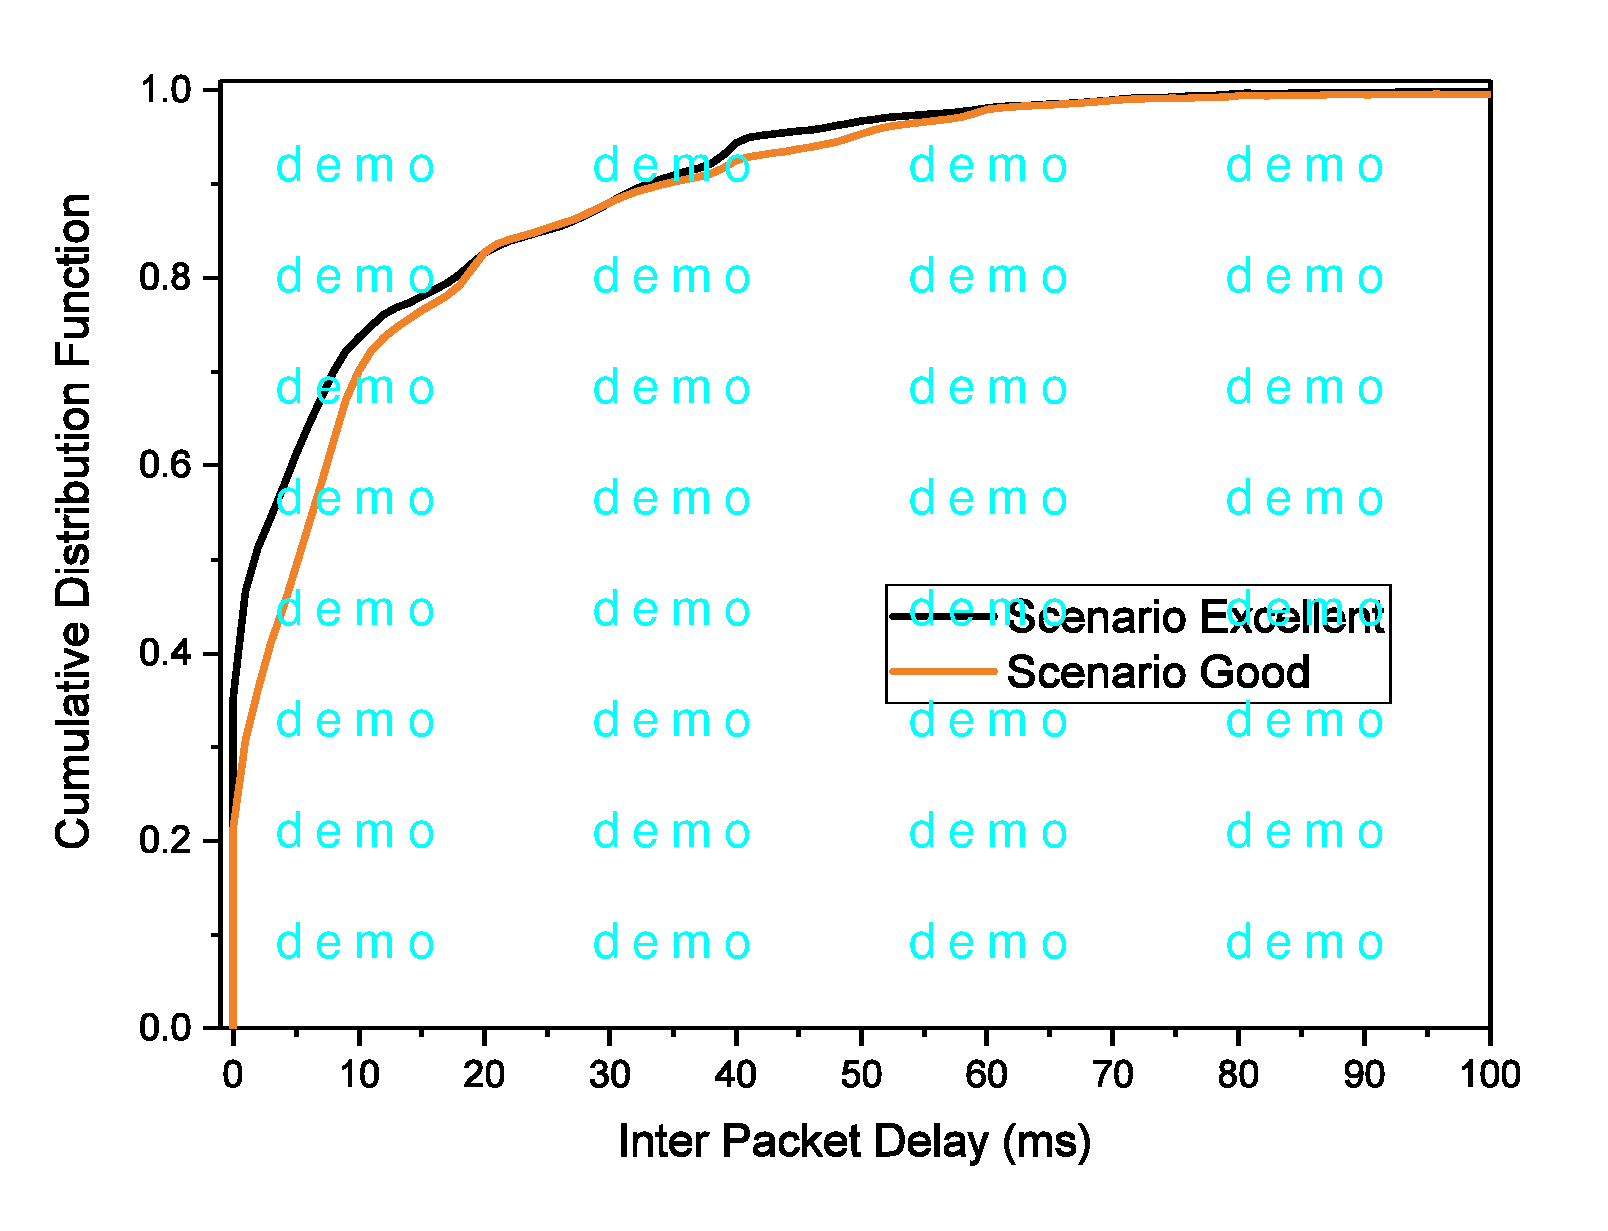
\includegraphics[width=0.48\textwidth]{chapters/chapter3/figures/capture-ipd-cdf.pdf}
        }
        \subfigure[IPD分布的概率密度函数图]{
            \label{fig:3:capture:ipd:pmf}
            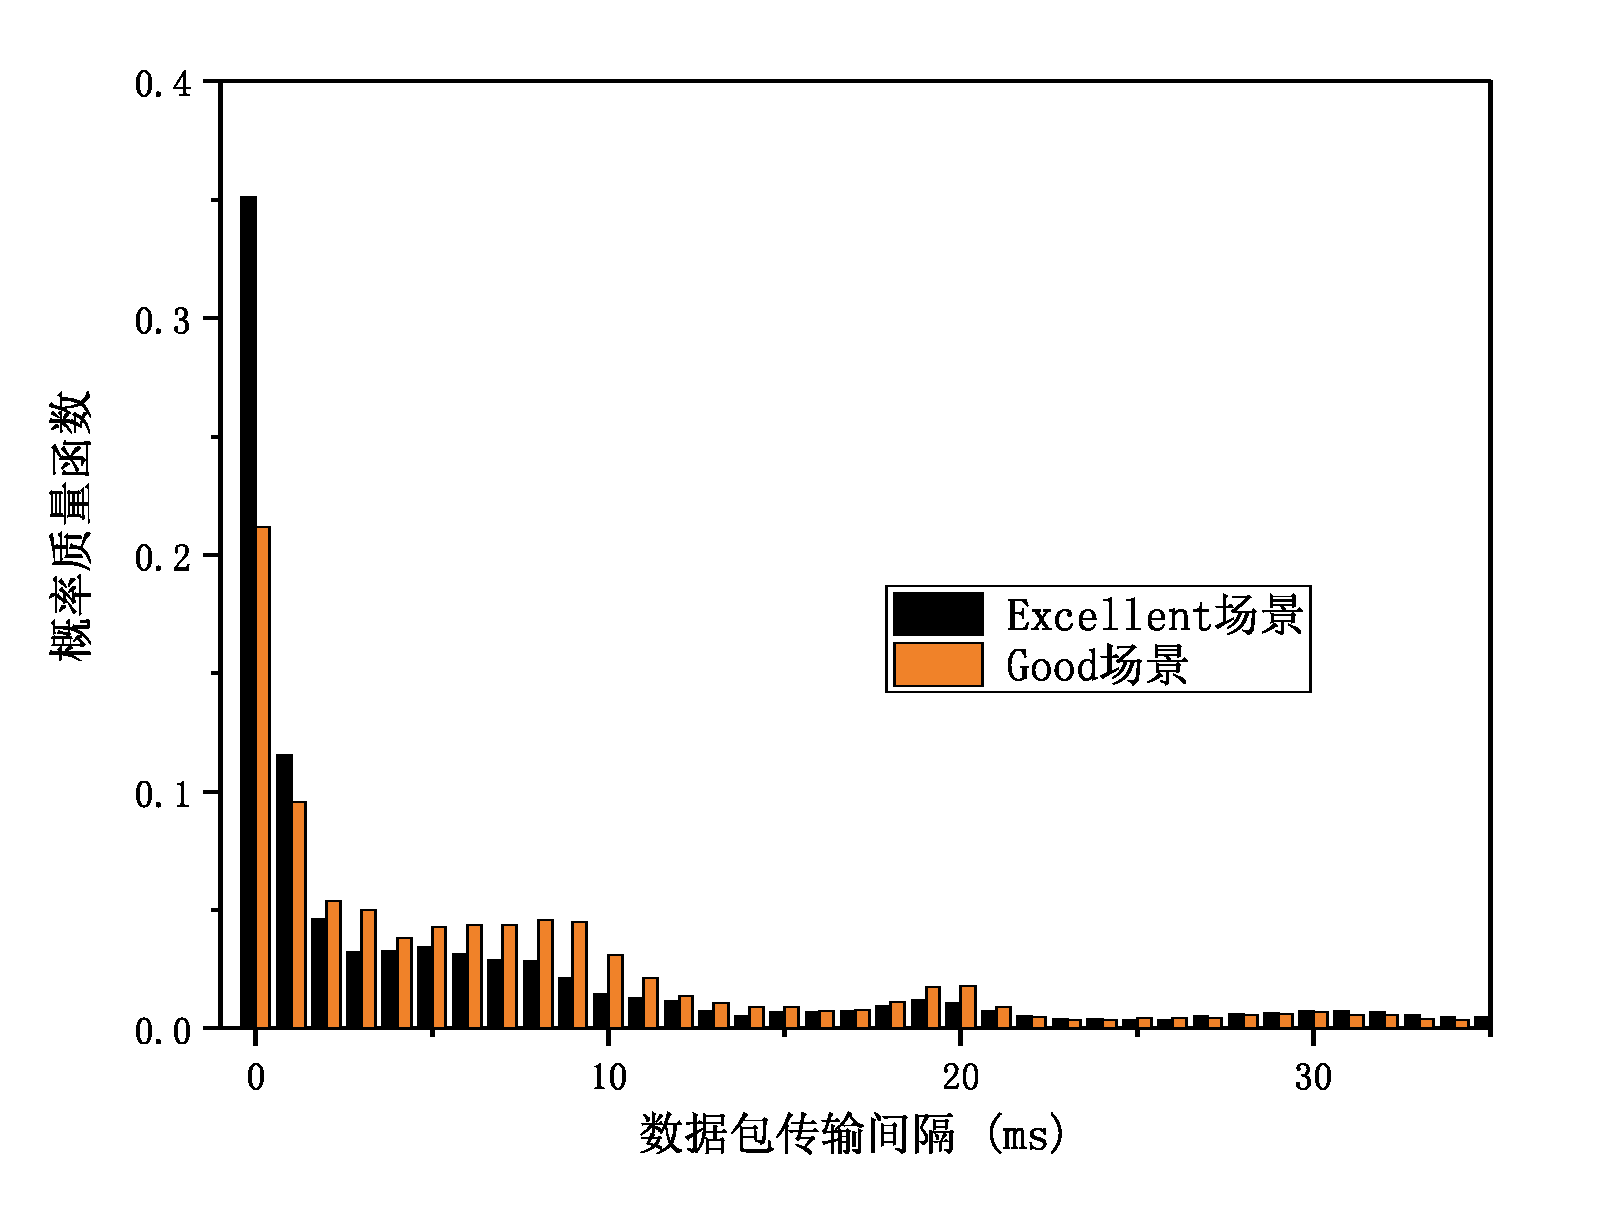
\includegraphics[width=0.48\textwidth]{chapters/chapter3/figures/capture-ipd-pmf.pdf}
        }
    \caption{VoLTE视频数据包IPD分布图}
    \label{fig:3:capture:ipd}
    \end{figure}
}

图\nref{fig:3:capture:ipd}中,分别展示了两种场景下的IPD分布情况。根据累积分布函数曲线,如图\nref{fig:3:capture:ipd:cdf},两种场景的趋势及数值范围均近似,证明丢包事件对IPD分布的影响,在总体分布中不明显。图\nref{fig:3:capture:ipd:pmf}中,PMF只显示了$IPD<35$的部分,对于$IPD \geq 35$的部分,二者没有显著差别。综合PMF及CDF的趋势,对基于主动丢包的时间隐通道来说,仅通过IPD分布检测是不完善的。另一方面,体现了该时间隐通道构建方法,在当前的检测方法面前具有较好的隐蔽性。

\subsection{突发丢包长度}
\label{chap:analyze:results:burst}

%什么是突发丢包长度
网络中的丢包事件,通常可以分为随机丢包和突发丢包,随机丢包为单个数据包随机丢失,突发丢包为多个数据包连续丢失。\nupcite{816237,6711984}。对于与基于VoIP的视频通话来说,随机丢包对视频质量产生的影响范围更广,突发丢包对视频稳定性影响更大。\nupcite{5977359,6894614,1709847}本文中,将随机丢包作为突发丢包的一种特征情况,即长度为1的突发丢包,进行统一的分布统计。

%两种场景下,测试得到的突发丢包长度信息
\insertFigure{
	\begin{figure}
		\centering
        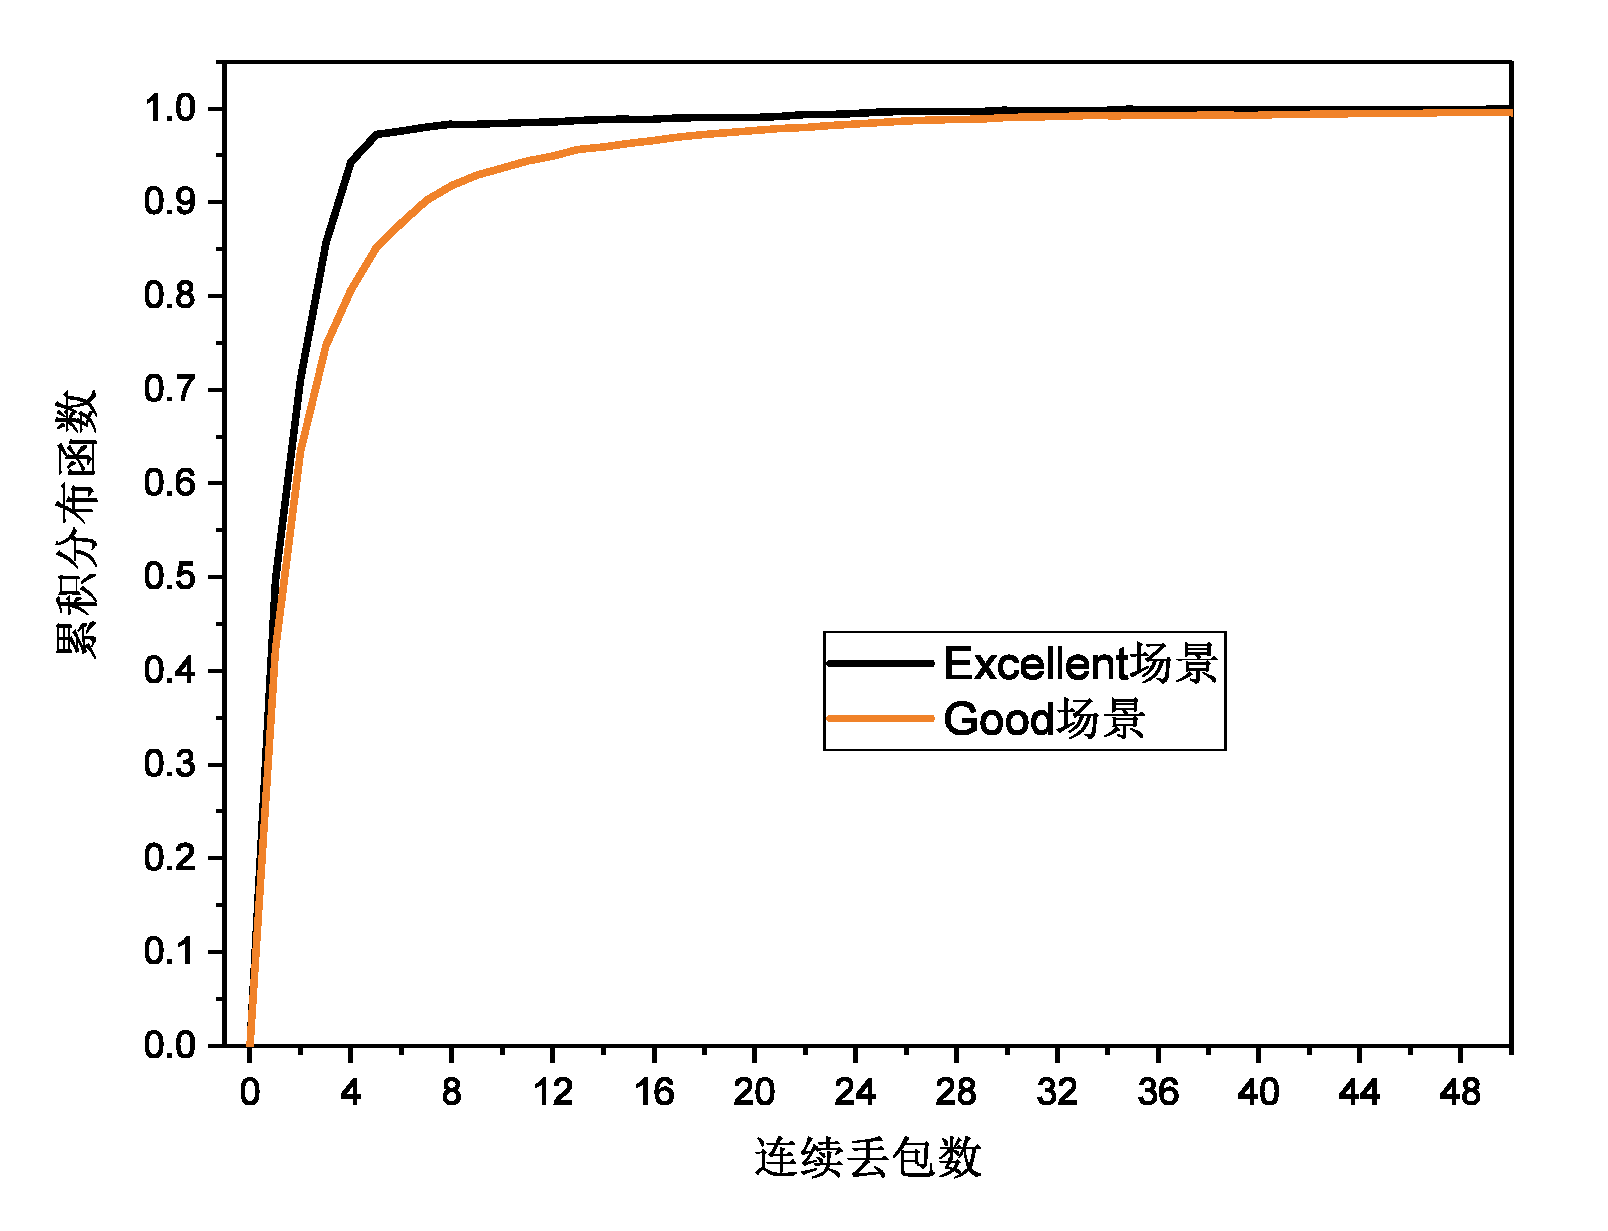
\includegraphics[width=0.75\textwidth]{chapters/chapter3/figures/capture-cdf-burst.pdf}
        \caption{两种场景中突发丢包长度的累积分布函数图}
        \label{fig:3:capture-cdf-burst}
	\end{figure}
}

如图\nref{fig:3:capture-cdf-burst},在两种网络场景中,突发长度的分布趋势趋于一致。具体到部分特征,Excellent场景与Good场景在$Burst\ Length > 1$的部分,在总体中的占比存在差异。在网络质量良好的场景中,突发丢包的长度非常短,累积分布函数曲线在其实阶段上升迅速。对于网络不稳定的场景,出现连续丢包现象,导致CDF曲线趋近1的速度减缓。当基于主动丢包的时间隐通道构造后,产生突发长度为1的丢包,对突发长度的分布曲线存在影响。